\documentclass[conference]{IEEEtran}
\IEEEoverridecommandlockouts

\usepackage{cite}
\usepackage{amsmath,amssymb,amsfonts}
\usepackage{graphicx}
\usepackage{booktabs}
\usepackage{tikz}
\usetikzlibrary{positioning,arrows.meta,calc}
\usepackage{textcomp}
\usepackage{xcolor}

\begin{document}

\title{Optimize Against EA: A Web-Based Game Suite\\ for Experiencing Evolutionary Optimization\\
{\footnotesize Game Lab II project report, Julius-Maximilians-Universit\"at W\"urzburg}
}

\author{
\IEEEauthorblockN{Philipp Sehne}
\IEEEauthorblockA{\textit{Games Engineering} \\
\textit{Julius-Maximilians-Universit\"at W\"urzburg}\\
W\"urzburg, Germany \\
Matriculation No.\ XXXXXXX}
\and
\IEEEauthorblockN{David Ahrens}
\IEEEauthorblockA{\textit{Games Engineering} \\
\textit{Julius-Maximilians-Universit\"at W\"urzburg}\\
W\"urzburg, Germany \\
Matriculation No.\ XXXXXXX}
}

\maketitle

\begin{abstract}
Evolutionary algorithms (EAs) are widely used black-box optimizers, yet the people who must sign off on decisions produced by such systems often have no intuition for how they search, improve, and sometimes fail. We present \emph{Optimize Against EA}, a freely accessible web application in which players compete against, observe, and configure a genetic algorithm across three mini-games: \emph{Peak Finder}, a probing race over continuous benchmark landscapes; \emph{Maze Explorer}, a combinatorial path-evolution sandbox; and a \emph{Shooter} in which a population of enemy agents evolves its behaviour against the player in real time. The project was developed in a user-centered engineering (UCE) process with a domain-expert stakeholder from the Organic Computing group at the University of Augsburg: an initial requirements interview, an intermediate quality gateway with a discarded first prototype, informal playtests, and a final evaluation shaped the product at every stage. We describe this process, the resulting requirements and system, and discuss what the artefact demonstrates --- and what it does not. In the stakeholder's final evaluation, the solution was rated as solving the problem and as ``easy and fun to work with,'' while the open question of whether it measurably \emph{teaches} EA behaviour is identified as the main direction for follow-up work.
\end{abstract}

\begin{IEEEkeywords}
evolutionary algorithms, genetic algorithms, serious games, game-based learning, user-centered design, black-box optimization
\end{IEEEkeywords}

\section{Introduction}
AI-based systems increasingly produce solutions --- schedules, shapes, parameters, policies --- that human stakeholders must approve and take responsibility for. An informed sign-off requires at least a working intuition for how the underlying optimizer behaves: how quickly it improves, how close to optimal its result plausibly is, and how its search can be misled. One important class of such optimizers are evolutionary algorithms (EAs), population-based metaheuristics that are routinely applied when the objective function is a black box, no dedicated solver exists, or the evaluation budget is limited \cite{eiben2015,holland1992}.

Intuition for EA behaviour is usually built by studying convergence plots and behaviour measures such as final quality, quality after a fraction of the budget, rate of improvement, or population diversity. For non-experts --- our stakeholder's stated target audience are adults in vocational training with no prior exposure to optimization --- this presentation is inaccessible. The premise of this project, proposed by Dr.\ Michael Heider (Organic Computing group, University of Augsburg) under the title \emph{``Are You Smarter Than Evolution?''}, is that these concepts can instead be \emph{experienced}: a player who races an EA on the same unknown function, with the same evaluation budget, feels first-hand how hard black-box optimization is and what the algorithm's improvement curve means.

Our contribution is \emph{Optimize Against EA}, a client-side web application built with React/TypeScript and hosted on Firebase, deliberately requiring no installation so it can be handed to a lecture audience or a curious layperson via a URL. The deliverable is the website as a whole: three games that expose the same underlying genetic algorithm (GA) from three angles, a dashboard, an ``EA Explained'' teaching section, and a shared hint system. Beyond the artefact itself, this report documents the user-centered engineering process that produced it (Section~\ref{sec:uce}), including the final requirements diagram and the stakeholder's questionnaire answers, and closes with an honest discussion of scope and limitations (Section~\ref{sec:discussion}) and the individually invested effort (Section~\ref{sec:workload}).

\section{Related Work}
\textbf{Human-vs-algorithm optimization games.} The direct inspiration, named in the project pitch, is Tobias Glasmacher's GECCO competition demo, a web interface in which a human selects probe points on a hidden 2D function and is scored against an optimizer. Our Peak Finder game adopts this core loop --- click-to-probe on a hidden continuous landscape under a shared budget --- and extends it with a configurable GA opponent, difficulty presets, and a post-game replay of the algorithm's generations. More broadly, human-guided and human-in-the-loop search has been studied as a means of combining human intuition with algorithmic throughput \cite{anderson2000,takagi2001}; our setting inverts the framing: the human is not steering the optimizer but competing with it, so that the optimizer's behaviour becomes the object of study.

\textbf{Benchmark functions.} The continuous problems in Peak Finder are drawn largely from the BBOB test suite of the COCO benchmarking platform \cite{hansen2021coco}, which the stakeholder pointed us to as a source of ``maps'': among the fourteen implemented functions are Sphere, Linear Slope, Sharp Ridge, Step-Ellipsoid, Attractive Sector, Rosenbrock, Ackley, Rastrigin, Schwefel, and Gallagher's 101 Peaks, complemented by classical test functions such as Booth, Beale, Bukin N.6, and Eggholder. Using an established suite means the difficulty characteristics of each map (multimodality, ill-conditioning, deceptive global structure) are well understood.

\textbf{Serious games and game-based learning.} Digital games have long been used to make formal or abstract material explorable \cite{prensky2001,gee2003}, and gamification research suggests that game elements such as competition and immediate feedback support engagement \cite{deterding2011}. Teaching-oriented visualizations of evolutionary computation exist mostly as non-interactive applets or lecture demos; to our knowledge, a freely accessible suite in which laypeople \emph{play against} and \emph{reconfigure} the same GA across continuous, combinatorial, and behavioural domains is not otherwise available. The stakeholder did not require citation of further specific systems.

\section{User-Centered Engineering Process}
\label{sec:uce}

\subsection{Stakeholder and process overview}
The sole stakeholder was Dr.\ Michael Heider (University of Augsburg, Organic Computing) in the role of the client and domain expert; course supervision was provided by Prof.\ Dr.\ Sebastian von Mammen. The process followed the Game Lab UCE structure: an initial requirements meeting, a requirements-modelling workshop, an intermediate \emph{quality gateway} at which the stakeholder formally assessed requirements and approach, iterative development with informal playtesting, and a final evaluation meeting with a closing questionnaire. The project ran from October 2025 (pitch dated 29 September 2025) to July 2026.

\subsection{Requirements elicitation (November 2025)}
The kickoff interview took place on 13 November 2025. Its minutes fixed the constraints that shaped all later design work: the target audience are \emph{adults without any prior contact with EAs or optimization}, typically with vocational rather than academic backgrounds (12--14-year-olds as an optional secondary audience); the genre should be \emph{simulation-flavoured mini-games} but explicitly not a bare simulation; topic delivery should use \emph{small feedback during play and a larger ``replay summary'' at the end}, without interrupting the flow of the game; player actions must always produce legible feedback, even while the player is still ``lost'' with respect to the optimization concepts; and \emph{arcade over narrative} --- mechanics take priority over story framing. These points map directly onto the final product: every game ends in a replay/recap view of the EA's generations, and none of the games carries narrative framing.

From the pitch and this interview we derived the requirements model shown in Fig.~\ref{fig:req}, first sketched in the course requirements workshop and consolidated at the end of the project. Five stakeholder requirements (STR1--STR5: convey EAs to laypeople; make optimization playful; free access for anyone; show the strength of EAs; work as a pastime) give rise to six derived system requirements --- an installation-free web platform, a player-customizable EA, a suite of optimization problems, competitive games against the EA, replay/recap feedback, and embedded teaching material and guidance --- each of which is satisfied by concrete design decisions, from the React/TypeScript stack down to the three mini-games and the hint system. During development, requirements were tracked without formal MoSCoW priorities (the IDs in Fig.~\ref{fig:req} were introduced when consolidating the final diagram); verification happened through the stakeholder-facing milestones described below rather than through a formal requirements table.

\begin{figure*}[t]
\centering
\resizebox{\textwidth}{!}{%
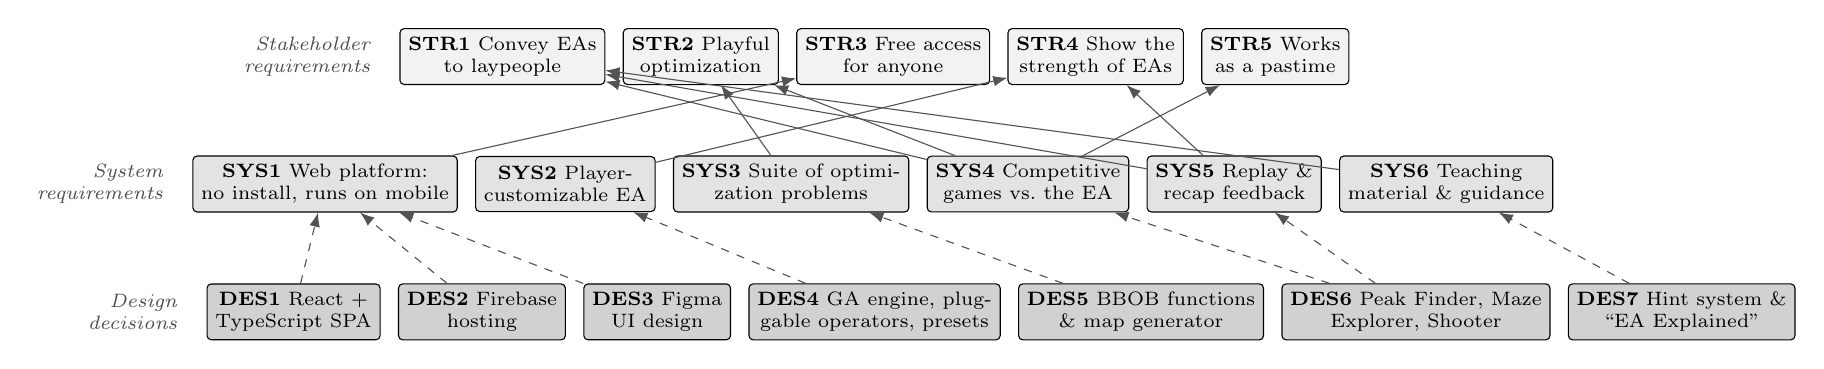
\begin{tikzpicture}[
  font=\scriptsize,
  req/.style={draw, rounded corners=1.5pt, align=center, inner sep=3pt, minimum height=7mm},
  str/.style={req, fill=gray!10},
  sys/.style={req, fill=gray!22},
  des/.style={req, fill=gray!36},
  tier/.style={font=\scriptsize\itshape, align=right, text=gray!60!black},
  derive/.style={-{Latex[length=1.8mm]}, gray!65!black, thin},
  satisfy/.style={-{Latex[length=1.8mm]}, gray!65!black, thin, dashed},
  node distance=9mm and 2.2mm
]
% ---- System requirements (middle tier, placed first for alignment) ----
\node[sys] (y1) {\textbf{SYS1} Web platform:\\no install, runs on mobile};
\node[sys, right=of y1] (y2) {\textbf{SYS2} Player-\\customizable EA};
\node[sys, right=of y2] (y3) {\textbf{SYS3} Suite of optimi-\\zation problems};
\node[sys, right=of y3] (y4) {\textbf{SYS4} Competitive\\games vs.\ the EA};
\node[sys, right=of y4] (y5) {\textbf{SYS5} Replay \&\\recap feedback};
\node[sys, right=of y5] (y6) {\textbf{SYS6} Teaching\\material \& guidance};
% ---- Stakeholder requirements (top tier) ----
\node[str, above=of y2, xshift=-8mm] (s1) {\textbf{STR1} Convey EAs\\to laypeople};
\node[str, right=of s1] (s2) {\textbf{STR2} Playful\\optimization};
\node[str, right=of s2] (s3) {\textbf{STR3} Free access\\for anyone};
\node[str, right=of s3] (s4) {\textbf{STR4} Show the\\strength of EAs};
\node[str, right=of s4] (s5) {\textbf{STR5} Works\\as a pastime};
% ---- Design decisions (bottom tier) ----
\node[des, below=of y1, xshift=-4mm] (d1) {\textbf{DES1} React +\\TypeScript SPA};
\node[des, right=of d1] (d2) {\textbf{DES2} Firebase\\hosting};
\node[des, right=of d2] (d3) {\textbf{DES3} Figma\\UI design};
\node[des, right=of d3] (d4) {\textbf{DES4} GA engine, plug-\\gable operators, presets};
\node[des, right=of d4] (d5) {\textbf{DES5} BBOB functions\\\& map generator};
\node[des, right=of d5] (d6) {\textbf{DES6} Peak Finder, Maze\\Explorer, Shooter};
\node[des, right=of d6] (d7) {\textbf{DES7} Hint system \&\\``EA Explained''};
% ---- Tier labels ----
\node[tier, anchor=east] at ($(s1.west)+(-2.5mm,0)$) {Stakeholder\\requirements};
\node[tier, anchor=east] at ($(y1.west)+(-2.5mm,0)$) {System\\requirements};
\node[tier, anchor=east] at ($(d1.west)+(-2.5mm,0)$) {Design\\decisions};
% ---- deriveReqt: system reqs derived from stakeholder reqs (arrow to source) ----
\draw[derive] (y1) -- (s3);
\draw[derive] (y2) -- (s4);
\draw[derive] (y3) -- (s2);
\draw[derive] (y4) -- (s1);
\draw[derive] (y4) -- (s2);
\draw[derive] (y4) -- (s5);
\draw[derive] (y5) -- (s1);
\draw[derive] (y5) -- (s4);
\draw[derive] (y6) -- (s1);
% ---- satisfy: design decisions satisfy system reqs (arrow to requirement) ----
\draw[satisfy] (d1) -- (y1);
\draw[satisfy] (d2) -- (y1);
\draw[satisfy] (d3) -- (y1);
\draw[satisfy] (d4) -- (y2);
\draw[satisfy] (d5) -- (y3);
\draw[satisfy] (d6) -- (y4);
\draw[satisfy] (d6) -- (y5);
\draw[satisfy] (d7) -- (y6);
\end{tikzpicture}}
\caption{Final requirements diagram (SysML-style). Solid arrows denote \textsf{\footnotesize$\langle\!\langle$deriveReqt$\rangle\!\rangle$} --- each system requirement points to the stakeholder requirement(s) it was derived from; dashed arrows denote \textsf{\footnotesize$\langle\!\langle$satisfy$\rangle\!\rangle$} --- each design decision points to the system requirement it realizes. Consolidated from the requirements workshop draft; SYS5 and SYS6 were added from the kickoff-interview constraints (replay summary, feedback, and explanation needs).}
\label{fig:req}
\end{figure*}

\subsection{Quality gateway and the discarded first prototype (January 2026)}
In mid-January 2026 we presented a first playable prototype: a game in which the player solved instances of the Travelling Salesperson Problem against the EA. The stakeholder's feedback at this milestone changed the product substantially. While he liked the website as a platform, he judged TSP to be a poor vehicle for \emph{visualizing} EA behaviour and asked instead for \emph{function approximation} on continuous landscapes --- the request from which Peak Finder was born. This is the clearest instance of feedback-driven redesign in the project: an entire game was dropped and replaced.

At the same meeting (video call, 16 January 2026) the stakeholder completed the \emph{Quality Gateway Questionnaire}. His answers were: \emph{``The stakeholder requirements represent our goals''} --- Agree; \emph{``We believe that the proposed approach solves our problem''} --- Strongly Agree; \emph{``The proposed workflow is attractive''} --- Agree. The gateway thus confirmed the (post-TSP) direction and the requirements model of Fig.~\ref{fig:req}.

\subsection{Playtesting (spring 2026)}
During development we ran informal playtests with fellow students and friends, focusing on whether the website's flow was understandable and the explanations sufficient. The consistent pattern: most testers initially struggled with Peak Finder and Maze Explorer --- several reported feeling ``scared'' of touching the EA settings or simply not understanding the parameters --- whereas the Shooter felt intuitive to almost everyone, and the enemies' generation-by-generation improvement was clearly perceived there. We reacted by adding a shared hint system, per-game tutorials, and safe difficulty presets (easy/normal/hard/expert) so that players never \emph{have} to open the full EA configuration to play.

\subsection{Final evaluation (July 2026)}
The final stakeholder meeting took place on 14 July 2026, with the finished website. The stakeholder's central concern, recorded in the minutes, was: \emph{do the games actually help players learn how a GA works?} Per game, he noted that in the Shooter one clearly sees \emph{that} something changes but not easily \emph{why} (suggesting to highlight which generations were good and why); that Peak Finder's randomly generated maps clustered their global optima (a map-generation bug we subsequently confirmed) and were too small, while the animation of generations converging on the target was singled out as good; and that Maze Explorer's controls were confusing in places and its ``experiment mode'' label sounded like a developer feature. Overall he asked for the ``EA Explained'' section to be formulated more abstractly, with each game then giving a concrete, game-specific instantiation. His summary judgement, verbatim from the minutes: \emph{satisfied with the solution, but unsure whether it actually works} --- i.e., whether it teaches.

He then completed the \emph{Final Evaluation Questionnaire} (signed 15 July 2026): \emph{``The communication was polite and professional''} --- Strongly Agree; \emph{``Our feedback was well-reflected''} --- Strongly Agree; \emph{``The delivered solution solves our problem''} --- Agree, annotated \emph{``Not sure if it trains well''}; \emph{``The delivered solution is easy and fun to work with''} --- Strongly Agree, annotated \emph{``Absolutely!''}. No requirement was formally rejected or deprioritized during the project; the scope adjustments that occurred (dropping TSP, deferring some scaffolded features) were reprioritizations agreed with the stakeholder.

\section{System}
\label{sec:system}
\textbf{Platform.} The system is a purely client-side single-page application (React, TypeScript, Vite) deployed on Firebase hosting. This was our call, motivated directly by the ``free access for anyone'' requirement: no download, no account, working on most devices including phones --- suitable for handing out in a lecture.

\textbf{The EA.} All three games are driven by a genetic algorithm whose configuration is exposed to the player: population size, number of generations, crossover rate, mutation rate, mutation strength, and mutation decay, plus a choice of selection strategy (tournament, roulette-wheel, or elitist), crossover operator (uniform, arithmetic, or single-point), and mutation operator (Gaussian, uniform, or Cauchy in the continuous games; point or segment mutation on the move sequence in Maze Explorer). We deliberately restricted the suite to GA variants rather than covering, e.g., evolution strategies --- one algorithm family, seen from many sides, seemed more digestible for the target audience.

\textbf{Peak Finder} implements the pitch's core idea: player and EA search the same hidden 2D landscape (one of the fourteen benchmark functions above, or a procedurally generated map) under comparable probe budgets; each player probe reveals a small neighbourhood of the surface, and after the race the player can step through every EA generation, inspect any generation's fitness, and watch a visualization of how offspring are produced from parents. \textbf{Maze Explorer} moves the same GA to a combinatorial domain: genomes are move sequences evolved to traverse a maze --- not a canonical optimization benchmark, but a deliberately legible one. \textbf{Shooter} embodies the EA rather than plotting it: enemy behaviour (aggression, movement speed, dodging, a cyclic movement pattern, even body size and opacity) is genome-encoded and evolves between waves against the player's own performance, so selection pressure is something the player \emph{causes}.

\textbf{Behaviour measures.} Of the measures suggested in the pitch, we surface fitness --- current, per generation, and as an improvement curve --- together with the interactive breeding visualization; diversity and rate-of-improvement are visible qualitatively in the replays but are not reported as explicit metrics.

\textbf{Technical obstacles.} We encountered three major obstacles. First, mobile performance: keeping per-frame simulation and rendering of full populations smooth on phones required significant optimization effort. Second, Shooter training dynamics: making the evolving enemies show \emph{visible, non-random} improvement within a session --- fitness shaping such that selection acts on genuinely better behaviour --- took considerable tuning. Third, fairness in Peak Finder: a single human competes against a population evaluating many candidates per generation; we balance via budgets and reveal radii, but a principled notion of a ``fair'' human-vs-population race remains open.

\section{Discussion}
\label{sec:discussion}
\textbf{What the project demonstrates.} The delivered website makes the mechanics of a genetic algorithm --- populations, selection, crossover, mutation, generational improvement --- observable and manipulable by laypeople in three complementary domains, at zero access cost. Playtesters consistently \emph{witnessed} the EA getting better, most strikingly in the Shooter; the stakeholder confirmed that the solution addresses his problem and is easy and fun to work with.

\textbf{What it does not prove.} We ran no formal evaluation of learning outcomes; whether players leave with a durably better understanding of EA behaviour --- the stakeholder's own final concern (``not sure if it trains well'') --- is an empirical question this project does not answer. Nor does the artefact showcase EAs at their best: Maze Explorer's problem is chosen for legibility, not for being a setting where a GA is the method of choice, and the restriction to a single algorithm family limits diversity. The pitch itself defers the most interesting claim --- that intuition gained on 2D landscapes transfers to higher-dimensional problems --- to follow-up work. A structured user study with pre/post concept tests, and the explanation-depth improvements requested in the final meeting (abstract overview plus game-specific instantiations, ``why was this generation good?''), are the natural next steps.

\section{Individual Workload}
\label{sec:workload}
The team consisted of two members who worked, for most of the project, in joint sessions and split the overall effort evenly ($\approx$50/50); hours were not formally tracked. Communication with the stakeholder --- all meetings and correspondence --- was carried jointly, as were design (concept, requirements, UI/UX in Figma), presentation, and documentation. Development was split by feature: Philipp Sehne owned Peak Finder and Maze Explorer; David Ahrens owned the Shooter games, the dashboard, and the main page; the hint system and the shared visual style were built together. Within presentation work, the poster was mainly David Ahrens's and the trailer mainly Philipp Sehne's. Cross-cutting decisions --- the user flow across the site, the website style, and technical features such as the hint system --- were made in joint sessions. Table~\ref{tab:workload} summarizes the split.

\begin{table}[t]
\caption{Distribution of effort per activity (shares of that activity).}
\label{tab:workload}
\centering
\begin{tabular}{@{}lcc@{}}
\toprule
Activity & P.\ Sehne & D.\ Ahrens \\
\midrule
Stakeholder communication & 50\,\% & 50\,\% \\
Design (concept, requirements, UI/UX) & 50\,\% & 50\,\% \\
Development: Peak Finder, Maze Explorer & 100\,\% & --- \\
Development: Shooter, dashboard, main page & --- & 100\,\% \\
Development: hint system, styles & 50\,\% & 50\,\% \\
Poster & minor & main \\
Trailer & main & minor \\
Report, handbook, documentation & 50\,\% & 50\,\% \\
\bottomrule
\end{tabular}
\end{table}

\section{Conclusion}
Optimize Against EA turns the abstract behaviour of a genetic algorithm into something a layperson can race, watch, and reconfigure in the browser. The user-centered process demonstrably shaped the product --- most visibly when the stakeholder's quality-gateway feedback replaced an entire TSP game with the function-approximation race he needed --- and his final evaluation endorses the result while marking its honest limit: the website makes EA behaviour \emph{experienceable}; showing that this experience \emph{teaches} is the follow-up study this project has prepared the ground for.

\section*{Acknowledgment}
We thank Dr.\ Michael Heider (University of Augsburg, Organic Computing) for proposing the project and for his engaged feedback throughout, and Prof.\ Dr.\ Sebastian von Mammen (Julius-Maximilians-Universit\"at W\"urzburg) for supervising the Game Lab.

\begin{thebibliography}{00}
\bibitem{eiben2015} A.~E. Eiben and J.~E. Smith, \emph{Introduction to Evolutionary Computing}, 2nd~ed. Berlin, Germany: Springer, 2015.
\bibitem{holland1992} J.~H. Holland, \emph{Adaptation in Natural and Artificial Systems}. Cambridge, MA, USA: MIT Press, 1992.
\bibitem{anderson2000} D.~Anderson, E.~Anderson, N.~Lesh, J.~Marks, B.~Mirtich, D.~Ratajczak, and K.~Ryall, ``Human-guided simple search,'' in \emph{Proc. AAAI}, 2000, pp. 209--216.
\bibitem{takagi2001} H.~Takagi, ``Interactive evolutionary computation: Fusion of the capabilities of EC optimization and human evaluation,'' \emph{Proc. IEEE}, vol.~89, no.~9, pp. 1275--1296, 2001.
\bibitem{hansen2021coco} N.~Hansen, A.~Auger, R.~Ros, O.~Mersmann, T.~Tu\v{s}ar, and D.~Brockhoff, ``COCO: A platform for comparing continuous optimizers in a black-box setting,'' \emph{Optimization Methods and Software}, vol.~36, no.~1, pp. 114--144, 2021.
\bibitem{prensky2001} M.~Prensky, \emph{Digital Game-Based Learning}. New York, NY, USA: McGraw-Hill, 2001.
\bibitem{gee2003} J.~P. Gee, \emph{What Video Games Have to Teach Us About Learning and Literacy}. New York, NY, USA: Palgrave Macmillan, 2003.
\bibitem{deterding2011} S.~Deterding, D.~Dixon, R.~Khaled, and L.~Nacke, ``From game design elements to gamefulness: Defining `gamification','' in \emph{Proc. 15th Int. Academic MindTrek Conf.}, 2011, pp. 9--15.
\end{thebibliography}

\end{document}
